%\documentclass[doubleblind]{ecai}  % use option [doubleblind] for double blind submission and hiding the authors section
\documentclass{ecai}
\usepackage{latexsym}
\usepackage{amssymb}
\usepackage{amsmath}
\usepackage{amsthm}
\usepackage{booktabs}
\usepackage{enumitem}
\usepackage{graphicx}
\usepackage{color}
\usepackage{multirow}
\usepackage{algorithm}
\usepackage{algpseudocode}
\usepackage{caption}
\usepackage{latexsym}

%%% Define any theorem-like environments you require here.

\newtheorem{theorem}{Theorem}
\newtheorem{lemma}[theorem]{Lemma}
\newtheorem{corollary}[theorem]{Corollary}
\newtheorem{proposition}[theorem]{Proposition}
\newtheorem{fact}[theorem]{Fact}
\newtheorem{definition}{Definition}

\setlength{\abovecaptionskip}{1pt}
\setlength{\belowcaptionskip}{1pt}

\begin{document}

\begin{frontmatter}

\title{Dynamic Multimodal Prompt Tuning: Boost Few-shot Learning with VLM-Guided Point Cloud Models}

\paperid{2932}
%this should be filled at the final stage, currently the submission doesn't include this.
\author[A]{\fnms{Xiang}~\snm{Gu}}
\author[A]{\fnms{Shuchao}~\snm{Pang}\orcid{0000-0002-5668-833X}\thanks{Corresponding Authors. \\Emails: pangshuchao@njust.edu.cn, anan.du@niit.edu.cn.}}
\author[B]{\fnms{Anan}~\snm{Du}\orcid{0000-0002-9634-3125}\footnotemark[*]}
\author[A]{\fnms{Yifei}~\snm{Wang}} 
\author[A]{\fnms{Jixiang}~\snm{Miao}}  
\author[C]{\fnms{Jorge}~\snm{Díez}\orcid{0000-0002-1314-2441}} 

\address[A]{School of Cyber Science and Engineering, Nanjing University of Science and Technology, China}
\address[B]{Nanjing Vocational University of Industry Technology, China}
\address[C]{Artificial Intelligence Center, University of Oviedo at Gijón, Spain}

   
\begin{abstract}
Few-shot learning is crucial for downstream tasks involving point clouds, given the challenge of obtaining sufficient datasets due to extensive collecting and labeling efforts. Pre-trained VLM-Guided point cloud models, containing abundant knowledge, can compensate for the scarcity of training data, potentially leading to very good performance. However, adapting these pre-trained point cloud models to specific few-shot learning tasks is challenging due to their huge number of parameters and high computational cost. To this end, we propose a novel Dynamic Multimodal Prompt Tuning method, named DMMPT, for boosting few-shot learning with pre-trained VLM-Guided point cloud models. Specifically, we build a dynamic knowledge collector capable of gathering task- and data-related information from various modalities. Then, a multimodal prompt generator is constructed to integrate collected dynamic knowledge and generate multimodal prompts, which efficiently direct pre-trained VLM-guided point cloud models toward few-shot learning tasks and address the issue of limited training data. Our method is evaluated on benchmark datasets not only in a standard N-way K-shot few-shot learning setting, but also in a more challenging setting with all classes and K-shot few-shot learning. Notably, our method outperforms other prompt-tuning techniques, achieving highly competitive results comparable to full fine-tuning methods while significantly enhancing computational efficiency.

\end{abstract}

\end{frontmatter}

\section{Introduction}

In the field of computer vision, 3D point cloud tasks are vital, with widespread applications in various areas like autonomous driving and robotics~\cite{chen2023fastc, bualașa2021lidar,du2024pcl}. 
%However, obtaining enough datasets for 3D point cloud tasks is challenging due to the cost and effort involved in collecting and labeling high-quality samples. Especially, this limits the performance of deep learning models. Hence, there is a need to design advanced methods that teach models to learn effectively from limited training data, known as few-shot learning. 
However, obtaining sufficient datasets for 3D point cloud tasks is challenging due to the cost and effort involved in collecting and labeling high-quality samples, which especially limits the performance of deep learning models.
Hence, there is a need to design advanced methods that teach models to learn effectively from limited training data \cite{pang2022beyond,pang2021tumor,lu2024uniads}, known as few-shot learning.
In the image field, pre-trained Vision Language Models (VLM), such as CLIP~\cite{radford2021learning}, have demonstrated strong capabilities in zero-shot and few-shot learning. 
%These models possess extensive knowledge in the image domain and are effectively aligned with text, making them promising for knowledge transfer to 3D tasks to help perform large-scale 3D representation learning. 
These models have very good performance in the image domain and are effective in working with text, which makes them promising for knowledge transfer to 3D tasks, for example, to help perform large-scale 3D representation learning.
Inspired by it, very recent studies have been dedicated to applying VLMs to 3D tasks~\cite{zhang2022pointclip,zhu2023pointclip,xue2023ulip,zhang2023uni3d}.
%~\cite{zhang2022pointclip}~\cite{zhu2023pointclip}~\cite{xue2023ulip}~\cite{zhang2023uni3d}.
%By using text-image-point triplet dataset~\cite{xue2023ulip}~\cite{deitke2023objaverse}
By using a data set with triplets of text, image and points~\cite{xue2023ulip,deitke2023objaverse} 
to align the 3D point encoder with pre-trained VLM's text encoder and vision encoder, VLM-Guided point cloud models, such as Uni3d~\cite{zhang2023uni3d} and ULIP~\cite{xue2023ulip}, are able to perform various downstream tasks in 3D fields. The abundant knowledge within pre-trained VLM-Guided point cloud models can compensate for the scarcity of training data, potentially leading to high performance in few-shot learning. However, these models contain a mixture of knowledge for multiple tasks, which implies that they need appropriate guidance to achieve good performance in specific few-shot learning tasks.

\begin{figure}[t]
\centerline{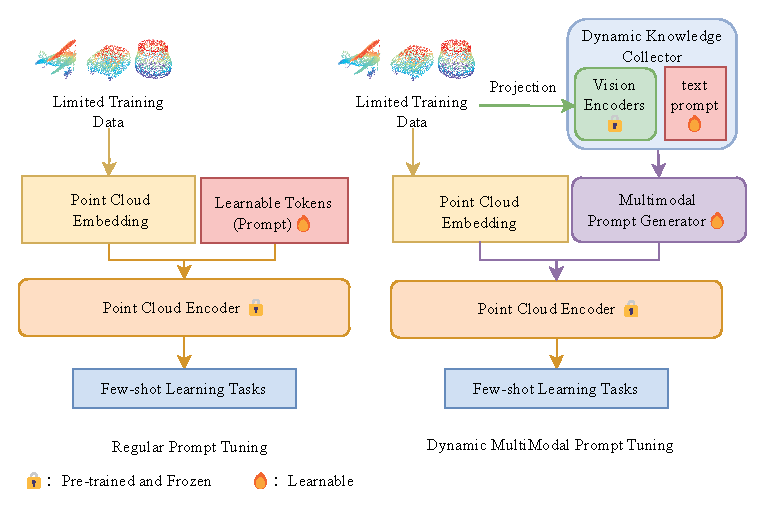
\includegraphics[width=0.95\linewidth]{compare.eps}}
% \captionsetup{font={footnotesize}, justification=raggedright}
\caption{Comparison with regular prompt tuning method: By collecting knowledge across modalities and generating dynamic multimodal prompts, we facilitate information sharing between modalities, empowering the point cloud encoder with additional knowledge to overcome the scarcity of training data.} \label{compare}
\vspace{4pt}
\end{figure}

%Researchers have explored two main approaches to realize pre-trained cloud models' full potential in few-shot learning tasks: 
Researchers have explored two main approaches to exploit the full potential of pre-trained cloud models in few-shot learning tasks:
fine-tuning~\cite{wang2023take, qi2023contrast, palakodety2020mining} and prompt tuning~\cite{jia2022visual, zha2023instance}. While fine-tuning is straightforward and commonly used, it is parameter-inefficient and can lead to overfitting-related problems, particularly with limited data available. In contrast, prompt tuning is introduced, which adds learnable tokens to guide the model; it doesn't change any parameters in pre-trained encoders and can reduce the risk of overfitting. In the 3D field, although there are some researches related to prompt tuning~\cite{hegde2023clip,zhu2023pointclip,zha2023instance}, they are limited to a single modality of a single encoder, wasting rich knowledge from other pre-trained encoders across different modalities. Moreover, this will trigger issues when the single pre-trained point cloud encoder lacks information about the target class, making it challenging to generate a proper prompt with limited data.



In order to address the above problems within the prompt tuning approach, inspired by the good performance of MaPle~\cite{khattak2023maple} in the 2D image field, we suppose that integrating knowledge from pre-trained encoders across different modalities can provide additional information, which is particularly beneficial when the current point encoder lacks relevant knowledge. Therefore, we propose the Dynamic Multimodal Prompt Tuning method, called DMMPT, for few-shot learning on 3D point clouds. In detail, we first construct a dynamic knowledge collector capable of leveraging encoders from diverse modalities to gather extra knowledge of the data and the targeted few-shot task. Based on it, we then propose a multimodal prompt generator that is able to take the dynamic knowledge collected via information bridges and generate a multimodal prompt. As shown in Figure~\ref{compare}, compared with regular prompt tuning methods, the proposed DMMPT method offers the ability to absorb knowledge of the training data in different modalities dynamically, and the generation of multimodal prompt enables better-guided information sharing between
modalities for few-shot learning tasks. Furthermore, our method does not edit any parameters in pre-trained encoders, making it significantly more efficient compared with fine-tuning-based methods. 
%In addition to the standard N-way K-shot few-shot learning setting, we also evaluate the proposed DMMPT method in a more challenging setting on benchmark datasets as described in PointCLIP~\cite{zhang2022pointclip}, where we sample K shots in each class. 
In addition to the standard N-way K-shot few-shot learning setting, we also evaluate the proposed DMMPT method in a more challenging setting, where we sample K shots in each class, following the learning setting presented by Zhang et al. in~\cite{zhang2022pointclip}.
In this setting, the trained model must learn to identify each class with relatively little data, which is closer to real-life applications. Even in such a few-shot learning setting, our DMMPT method continues to deliver very good performance.

Our main contributions are as follows:
\begin{enumerate}
    \item  We propose DMMPT, a new prompt tuning method for VLM-Guided point cloud models for few-shot learning. By introducing a dynamic knowledge collector capable of gathering knowledge from various modalities and creating a multimodal prompt generator to enhance knowledge sharing, we manage to fully absorb information across modalities and boost pre-trained point cloud models in few-shot learning tasks.
    \item We evaluate our model not only in the standard N-way K-shot few-shot settings but also in a challenging setting with a larger number of classes for models to identify. This highlights the potential of our method in real-life applications.
    \item Experiments demonstrate that our model exhibits outstanding performance in both few-shot learning settings. Our method outperforms other prompt-tuning-related methods and maintains strong competitiveness with full fine-tuning methods while significantly enhancing computational efficiency.
\end{enumerate} 

The remaining of the work is organized as follows: In the next section, the related work is discussed. Section~\ref{Methodology} introduces the details of DMMPT, the proposed method. Section~\ref{experiments} presents the experimental results and Section~\ref{ablation} is for the ablation study. Finally, conclusions are presented in Section~\ref{conclusion}.
%The work is concluded in Section~\ref{conclusion}.

\section{Related Work}
This section discusses the related work for the few-shot learning in point cloud field and VLM-Guided point cloud models as follows.
\subsection{Few-shot Learning in Point Cloud Model}
When it comes to few-shot learning in pre-trained VLM-Guided or self-supervised point cloud models, fine-tuning and prompt-tuning approaches are widely used. Among them, fine-tuning related methods~\cite{liu2023regress, wang2021unsupervised,yu2022point} exhibit good performance when parameters are fully fine-tuned. However, this approach not only requires abundant data but also incurs high computational costs, and it may even lead to overfitting issues. Additionally, it raises problems when there is a significant gap between the original tasks and the subsequent tasks. Instead, prompt tuning methods don't modify any parameters in pre-trained encoders, making them advantageous and efficient for dealing with small datasets. For example, PointCLIPV2~\cite{zhu2023pointclip} utilizes large language models to generate a text prompt that creates a semantic space closer to 3D scenes, representing an improvement in text prompts. CG3D~\cite{hegde2023clip}, learning from visual prompts in the image field, adds learnable tokens to the vision encoder to better align the 3D encoder and the pre-trained vision encoder. Moreover, some attempts are also made in 3D encoders. IDPT~\cite{zha2023instance}, introduced by Zha et al., applies Dynamic Prompt Tuning on pre-trained point cloud models, which generates prompts by capturing semantic prior features of each point cloud and demonstrates competitive performance compared with fine-tuning methods. However, all the methods mentioned are limited to prompts at a single modality. Prompting a single encoder may encounter difficulties when the pre-trained encoder lacks knowledge about the target class. To address this, we aim to combine the rich knowledge from pre-trained encoders across different modalities and utilize additional information to generate a multimodal prompt, enhancing overall performance.

\subsection{VLM-Guided Point Cloud Model}
The development of the VLM-Guided point cloud model progresses through two stages. Initially, researchers aim to project point clouds into depth images to fit the vision encoder. Subsequently, with the introduction of large-scale text-image-point triplet datasets, researchers propose a 3D encoder to align it with pre-trained vision-language models. 

In the first stage, aiming to transfer the rich knowledge from Vision Language Models (VLMs), PointCLIP~\cite{zhang2022pointclip} and PointCLIPV2~\cite{zhu2023pointclip} involves the direct projection of point clouds into depth maps from different angles. These depth maps are then fed into the CLIP vision encoder to perform zero-shot tasks. Similarly, Liu et al. propose PartSLIP~\cite{liu2023partslip}, which utilizes GLIP~\cite{li2022grounded} for low-shot part segmentation of 3D point clouds. Additionally, it employs multi-view feature fusion to enhance the transfer of point cloud features to the vision encoder. These methods employ projection techniques to convert 3D point clouds into a 2D field. However, during this process, crucial geometry features of the point cloud may be lost, and performance is influenced by the transformation of modalities.

\begin{figure*}[th]
\centerline{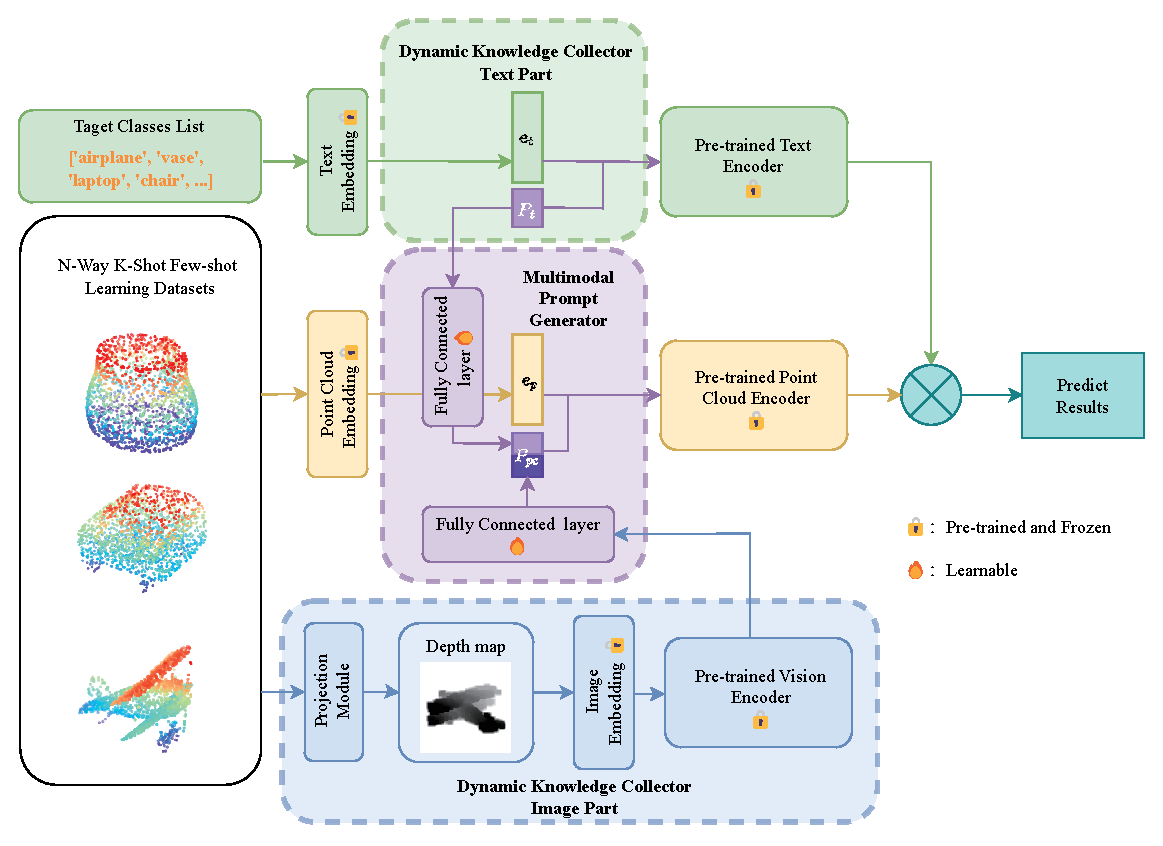
\includegraphics[width=0.95\linewidth]{pipeline.eps}}
% \captionsetup{font={footnotesize}, justification=raggedright}
\caption{The pipeline of Dynamic Multimodal Prompt Tuning (DMMPT): By introducing a dynamic knowledge collector and a multimodal prompt generator to gather and enable knowledge sharing across modalities, DMMPT fully leverages the information hidden in three modalities dynamically and efficiently without changing any parameters in pre-trained encoders. It achieves exciting performance with limited data in few-shot learning tasks.     } \label{pipeline}
\vspace{4pt}
\end{figure*}
     
In the second stage, 3D encoders are introduced to further narrow the domain gap between 2D images and 3D point clouds. Huang et al. introduce CLIP2Point~\cite{huang2023clip2point}, which employs a novel Gated Dual-Path Adapter to align with the CLIP vision encoder and effectively applies tuned pre-training knowledge to the following tasks. Recently, with advancements in the creation of large-scale text-image-point triplet datasets, ULIP~\cite{xue2023ulip}, proposed by Xue et al., enhances the alignment between the 3D point encoder and CLIP encoders. Zhou et al., in the proposal of UNI3D~\cite{zhang2023uni3d}, take a step forward by leveraging abundant 2D pre-trained models as initialization and employing scaling-up strategies to scale up Uni3D~\cite{zhang2023uni3d} to one billion parameters. While these models are powerful, it is too large to fine-tune them into downstream tasks, so their abundant knowledge needs further guidance to achieve better performance in subsequent tasks. To address this, we propose a prompt-based method designed to efficiently and dynamically facilitate information across modalities, enhancing the performance of VLM-Guided point cloud models.

\section{Methodology}\label{Methodology}
In this section, we will delve into the proposed dynamic knowledge collector and the multimodal prompt generator, as shown in Figure~\ref{pipeline}. Then, we will provide a detailed explanation of our pipeline.


\subsection{Preliminaries}
Typically, VLM-Guided point cloud models employ three encoders during training. They utilize the text encoder $f_T(\cdot)$ and image encoder $f_I(\cdot)$ from pre-trained vision language models and align the 3D encoder $f_P(\cdot)$ with them using text-image-point triplet datasets. During training, all three encoders are involved, but only the parameters in the 3D encoder are updated via cross-modal contrastive loss. At the inference stage, only two modalities are involved. Given a point cloud $P$ and target classes list $\{T_i\}_{i=1}^N$ with the class name of  $N$ classes, we got normalized features \begin{equation}\label{eqn-1} feat^{Text} = \frac{f_T(T)}{|f_T(T)|},\end{equation} and \begin{equation}\label{eqn-2} e^P = \frac{f_P(P)}{|f_P(P)|},\end{equation} so the resulting prediction is \begin{equation}\label{eqn-3} pred = argmax(e^P\cdot (feat^{Text})^T).\end{equation}

Motivated by the training process involving all three modalities, we aim to develop a dynamic multimodal prompt tuning method, which can leverage the potential knowledge in different pre-trained encoders across modalities to provide extra knowledge and further align the point cloud encoder and text encoder in few-shot learning tasks. Our method, Dynamic Multimodal Prompt Tuning (DMMPT), extracts knowledge from different modalities without editing any parameters in the pre-trained model and only requires a small amount of labeled data.

\subsection{Dynamic Knowledge Collector}
A dynamic knowledge collector is introduced to gather information across encoders of different modalities. It contains two parts, i.e., the text part and the image part, which serve as the task-related and the data-related knowledge collector respectively. The purpose of the dynamic knowledge collector is to help generate our dynamic multimodal prompt in the point branch.

In the text branch, we initialize the text prompt tokens $Prompt^T \in R^{n \times d_t}$, where $d_t$ represents the dimension of the text embedding, and $n$ denotes the prompt size. This text prompt conducts learnable prompt tuning in the text branch, enabling it to absorb task-related knowledge. Subsequently, this acquired knowledge will be integrated into the multimodal prompt generator, guiding the pre-trained point cloud encoder to specific few-shot learning tasks. We only require dataset class names as text inputs since the learnable text prompt tokens $Prompt^T$ are utilized, eliminating the need to preprocess the initial text input like PointCLIPV2~\cite{zhu2023pointclip}.

In the image branch, considering the flexibility of images, our purpose is to dynamically leverage image information into the point cloud branch to enhance the generation of point prompts by its additional data-related knowledge. To achieve this, we utilize the image features $feat^I$ processed by a pre-trained vision encoder $f_I(\cdot)$ and directly use it as a part of inputs for point prompt generation instead of adding additional learnable tokens like text prompt. In certain few-shot tasks, the original image paired with the point cloud may not be feasible. Consequently, we resort to projecting the point cloud into depth images from various views. We follow the same image projection method used
in PointCLIPV2~\cite{zhu2023pointclip} to project point cloud, which is parameter-free and requires point clouds only. The extensive knowledge provided by the pre-trained vision encoder gives huge benefits to boost the generation of the dynamic multimodal prompt with limited training data. 

\subsection{Dynamic Multimodal Prompt Generation}
After collecting task-related knowledge $Prompt^T$ and dynamic data-related knowledge $feat^I$ via our dynamic knowledge collector, we build a prompt generation module in the point cloud branch to absorb the rich and dynamic information provided by $Prompt^T$ and $feat^I$ and generate a point cloud prompt.

As for the learnable text prompt source $Prompt^T$, we employ fully connected layers to construct an information bridge $f_{T \rightarrow P}(\cdot)$ to bridge text prompt source $Prompt^T$ into point cloud dimension. Beyond offering knowledge to the point cloud branch, it also brings information back to the text branch to help prompt the text encoder. Thus we build a strong knowledge sharing between modalities and co-prompt them at the same time.

On the other hand, we choose to directly use image features $feat^I$ collected by dynamic knowledge collector. Based on our observation, we suppose that in the text encoder, the target classes are static so the input remains the same, making it easier to reach the target semantic space. However, image inputs are dynamic and complex so simply using learnable tokens can not provide useful information. Thus, we choose to use the whole image feature, which contains image information as the source to generate a point cloud prompt and feed it to a fully connected layer bridge $f_{I \rightarrow P}(\cdot)$ to bring dynamic and rich knowledge to the point cloud branch. Compared with training learnable tokens on the vision encoder, directly applying image features is parameter-free so it is much more efficient. 

The two bridges $f_{T \rightarrow P}(\cdot)$ and $f_{I \rightarrow P}(\cdot)$, individually transform $Prompt^T$ and $feat^I$ into the dimension of point cloud embedding. We concatenate them to initialize  $Prompt^{mul} \in R^{(n+1) \times d_{point}}$. Then we append $Prompt^{mul}$ at the end of point cloud embedding and randomly drop ($n+1$) in the point embedding to keep the total shape the same. By doing so, we are able to enhance the information communication between modalities and boost the prompt generation.

\subsection{Pipeline} 
Given a dataset of text, point cloud $\{T_i, P_i\}_{i=1}^N$, the first thing to do is to collect dynamic knowledge across modalities for multimodal prompt generation. In the text branch, we create a list $T$ consisting of all classes of the dataset and then obtain embedding features \begin{equation}\label{eqn-4} e^T = Embed_{text}(T). \end{equation} The text prompt tokens are $Prompt^T \in R^{n \times d_t}$, where $d_t$ represents the dimension of the text embedding, and $n$ denotes the prompt size. Then, we concatenate $e^T$ and our text prompt $Prompt^T$, and feed them into the pre-trained text encoder $f_T(\cdot)$ to obtain normalized text features \begin{equation}\label{eqn-5} feat^{Text} = \frac{f_T([e^T ,Prompt^T])}{|f_T([e^T ,Prompt^T])|}.\end{equation} 

In the image branch, we first project point clouds $\{P_i\}_{i=1}^N$ into depth maps $\{ I_i\}_{i=1}^N $. The final normalized image feature is directly achieved via a pre-trained vision encoder $f_I(\cdot)$. \begin{equation}\label{eqn-6} feat_i^{Image} = \frac{f_I(I_i)}{|f_I(I_i)|}.\end{equation} 

In the point cloud branch, we create two fully connected layers $f_{T \rightarrow P}(\cdot)$ and $f_{I \rightarrow P}(\cdot)$ to bridge text prompt and dynamic image features to point cloud branch, so point prompt is \begin{equation}\label{eqn-7} Prompt^P_i = [f_{T \rightarrow P}(Prompt^T),f_{I \rightarrow P}(feat_i^{Image})].\end{equation} Pre-trained embedding layer is used to get point cloud embedding \begin{equation}\label{eqn-8} e^P_i = Embed_{point}(P_i).\end{equation} Finally we get normalized point cloud features \begin{equation}\label{eqn-9} feat_i^{Point} = \frac{f_P([e^P_i,Prompt^P_i])}{|f_P([e^P_i,Prompt^P_i])|}.\end{equation}

Training purpose is to minimize cross entropy loss:\begin{equation}\label{eqn-10} Loss = Cross\_entropy(feat_i^{Point}\cdot( feat^{Text})^T,label).\end{equation} During training stage only parameters in text prompt $Prompt^T$ and two prompt bridges  $f_{T \rightarrow P}(\cdot)$, $f_{I \rightarrow P}(\cdot)$ are updated while parameters in pre-trained encoders are frozen. At inference stage, the predicted result is \begin{equation}\label{eqn-11} pred = argmax(feat_i^{Point}\cdot( feat^{Text})^T).\end{equation}

The whole algorithm of our method is shown in Algorithm \ref{alg}.
\begin{algorithm}
\caption{Dynamic Multimodal Prompt Tuning}
\label{alg}
\begin{algorithmic}[1]
\Require Few-shot learning dataset$\{T_i, P_i\}_{i=1}^N$, 
pre-trained encoders $f_T(\cdot)$, $f_I(\cdot)$, $f_P(\cdot)$
\Ensure Trained parameters $Prompt^T$, $f_{T \rightarrow P}(\cdot)$, $f_{I \rightarrow P}(\cdot)$
\State \textbf{Dynamic Knowledge Collector Text Part:} 
    \State $feat^{\text{Text}} \gets f_T([Embed_{\text{text}}(T), Prompt^T])$
\State \textbf{Dynamic Knowledge Collector Image Part:}
    \State$feat_i^{\text{Image}} \gets f_I(I_i)$
\State \textbf{Multimodal Prompt Generator:} 
    \State $Prompt^P_i \gets [f_{T \rightarrow P}(Prompt^T), f_{I \rightarrow P}(feat_i^{\text{Image}})]$
    \State $feat_i^{\text{Point}} \gets f_P([Embed_{\text{point}}(P_i), Prompt^P_i])$
\State \textbf{Training:} 
\State Minimize $Loss = \text{Cross\_entropy}(feat^{\text{Text}} \cdot (feat_i^{\text{Point}})^T, label)$
\State \textbf{Inference:} 
\State Predict result $pred = argmax(feat_i^{\text{Point}} \cdot (feat^{\text{Text}})^T)$
\end{algorithmic}
\end{algorithm}
\subsection{Pre-trained Models}
We utilize trained parameters from EVA~\cite{fang2023eva} as our pre-trained text and vision encoders, and from Uni3D~\cite{zhang2023uni3d} as our pre-trained point cloud embedding and point cloud encoder. For those datasets without paired images, the depth projection of each point cloud is created following the projection method in PointCLIPV2~\cite{zhu2023pointclip}; this is a direct depth projection from the point cloud, so this kind of image projection does not require extra data, which keeps it a fair comparison. 

\section{Experiments}\label{experiments}
In this section, we first introduce benchmark settings for few-shot learning tasks, including the standard N-way K-shot few-shot learning setting as well as few-shot learning with K-shot and all class settings. Subsequently, we explain the dataset used and its processing details. Following this, we present and analyze the outcomes of our experiments under the two few-shot learning settings respectively. Furthermore, we conduct t-SNE visualization to do a qualitative analysis of our method.

\subsection{Settings}
\subsubsection{Few-shot Learning Benchmark Settings}\label{Benchmark}
We train and evaluate our model under two different settings. 
The first setting is the standard N-way K-shot few-shot learning setting. We randomly select N classes from the entire set of classes and then sample K+20 points for each class. The training set (support set) consists of N $\times$ K samples, and the test set (query set) consists of the rest of N $\times$ 20 samples. We repeat this process T times to generate T folds containing different classes. Then the model is trained and evaluated on each fold separately. Finally, the accuracy is calculated as the average across all T folds. 

In the standard N-way K-shot few-shot learning setting, we compare our method with fine-tuning related methods, including OcCo~\cite{wang2021unsupervised}, Point-BERT~\cite{yu2022point}, Point-MAE~\cite{pang2022masked}, Point-M2AE~\cite{zhang2022point}, Point2vec~\cite{abou2023point2vec}, Point-RAE~\cite{liu2023regress}, TAP~\cite{wang2023take}, ReCon~\cite{qi2023contrast}, PointGPT~\cite{chen2024pointgpt}, and prompt tuning related methods which contain IDPT~\cite{zha2023instance} and ACT~\cite{dong2022autoencoders}.

We also evaluate our model in a more challenging setting with all classes following the settings of PointCLIP~\cite{zhang2022pointclip}. We call it few-shot learning with K-shot and all classes. In a dataset with N classes, K samples are randomly selected from each class, resulting in an $\text{N}\times \text{K}$ sample training set. We utilize the original test set of the dataset as our test set. This evaluation setting differs from the standard N way K shot few-shot setting in that it involves whole classes in the dataset, making it more challenging. 

In few-shot learning with K-shot and all-classes settings, we compare our model with methods mentioned in the same few-shot learning setting to keep a fair comparison. We use regular point cloud models including PointNet~\cite{qi2017pointnet}, PointNet++~\cite{qi2017pointnet++}, CurveNet~\cite{muzahid2020curvenet} and VLM-Guided models including SimpleView~\cite{goyal2021revisiting}, PointCLIP~\cite{zhang2022pointclip}, PointCLIPV2~\cite{zhu2023pointclip} as our baseline.

\subsubsection{Experimental Details}
We choose two widely-used benchmark datasets, ModelNet40~\cite{wu20153d} and ScanObjectNN~\cite{uy2019revisiting}, to evaluate our DMMPT method following the same settings from the compared methods. As shown in Figure~\ref{dataset}, ModelNet40 is a 40-categories dataset with synthetic object point clouds generated from CAD-generated meshes, which is clean and well-constructed. ScanObjectNN is a real-world dataset in 15 categories. Compared with ModelNet40, ScanObjectNN is close to real-world applications where the scanned point clouds have missing parts and deformations. We use the PB T50 RS split of ScanObjectNN as our source dataset for the generation of a few-shot learning dataset. 

\begin{figure}[t]
\centerline{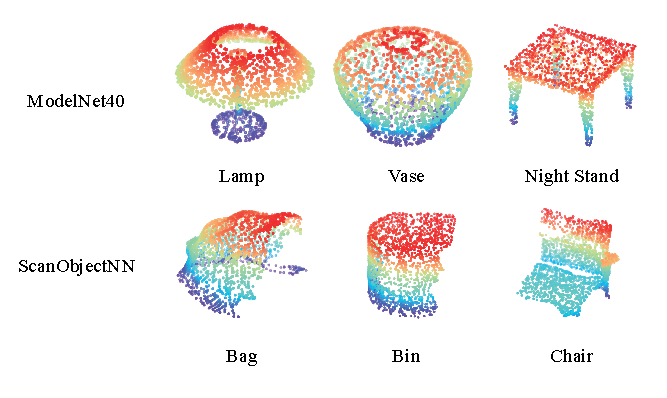
\includegraphics[width=0.95\linewidth]{dataset.eps}}
% \captionsetup{font={footnotesize}, justification=raggedright}
\caption{Some examples from used ModelNet40 and PB T50 RS split of ScanObjectNN datasets in our experiments. ModelNet40 is a 40-category synthetic object point cloud that is clean and well-constructed. ScanObjectNN is a real-world dataset in 15 categories, which has missing parts and deformations.}\label{dataset}
\vspace{4pt}
\end{figure}

In the standard N-way K-shot few-shot learning setting, we evaluate our model under ModelNet40. We directly use the ten-fold split following 
%PointBert~\cite{yu2022point} 
Yu et al.~\cite{yu2022point}
to make a fair comparison. In the few-shot learning setting with K-shot and all classes, we  
 train and evaluate our model on ModelNet40 and ScanObjectNN. The training data is randomly chosen from the original training dataset and we evaluate our model in the original test dataset. 

The hyper-parameters remain the same in each few-shot learning experiment. The text prompt size in the dynamic knowledge collector is set to 3, and the final multimodal prompt size is set to 4 in the multimodal prompt generator. The training epoch is 50 for each experiment. All experiments were conducted on a single NVIDIA A800 80 GB.
\subsection{Experimental Results}

\subsubsection{Standard N-way K-shot Few-shot Learning}
\begin{table*}
\begin{center}
% \captionsetup{font={footnotesize}}
{\caption{Comparisons with SOTA methods under Standard N-way K-shot few-shot learning on ModelNet40 benchmark dataset. We report the average classification accuracy (\%) with the standard deviation (\%) of 10 independent experiments. \#TP (M) denotes trainable parameters (million) in models in the fine-tuning or prompt-tuning stage.}\label{table1}}
\begin{tabular}{llccccc}
\toprule
&&\multicolumn{2}{c}{5 Way} & \multicolumn{2}{c}{10 Way} \\
\cline{3-6}
\\[-6pt]
&&\multicolumn{1}{c}{10 shot} & \multicolumn{1}{c}{20 shot} & \multicolumn{1}{c}{10 shot} & \multicolumn{1}{c}{20 shot} & \multicolumn{1}{c}{\#TP (M)} \\
\midrule
\multirow{9}{*}{\shortstack{Fine Tuning\\related methods}} 
&OcCo+PointNet~\cite{wang2021unsupervised}&89.7$\pm$1.9&92.4$\pm$1.6 &83.9$\pm$1.8 & 89.7$\pm$1.5& 22.1\\
&Point-BERT~\cite{yu2022point}& 94.6$\pm$3.1&96.3$\pm$2.7&91.0$\pm$5.4&92.7$\pm$5.1& 22.1\\
&Point-MAE~\cite{pang2022masked}&96.3$\pm$2.5&97.8$\pm$1.8&92.6$\pm$4.1&95.0$\pm$3.0& 22.1\\
&Point-M2AE~\cite{zhang2022point}&96.8$\pm$1.8&98.3$\pm$1.4&92.3$\pm$4.5&95.0$\pm$3.0& 15.3\\
&Point2vec~\cite{abou2023point2vec}& 97.0$\pm$2.8&98.7$\pm$1.2&93.9$\pm$4.1& 95.8$\pm$3.1&-\\
&Point-RAE~\cite{liu2023regress}& 97.3$\pm$1.6&98.7$\pm$1.3&93.3$\pm$4.0&95.8$\pm$3.0 &-\\
&TAP~\cite{wang2023take}&97.3$\pm$1.8&97.8$\pm$1.7&93.1$\pm$2.6&95.8$\pm$1.0& 12.6\\
&ReCon~\cite{qi2023contrast}&97.3$\pm$ 1.9&98.9$\pm$1.2&93.3$\pm$3.9&\textbf{98.9$\pm$1.2}& 44.3\\
&PointGPT~\cite{chen2024pointgpt}&\textbf{98.0$\pm$1.9}&99.0$\pm$1.0&94.1$\pm$3.3&96.1$\pm$2.8&>82.1\\
\midrule
\multirow{3}{*}{\shortstack{Prompt Tuning\\related methods}} 
&ACT~\cite{dong2022autoencoders}&96.8$\pm$2.3&98.0$\pm$1.4&93.3$\pm$4.0&95.6$\pm$2.8&22.1\\
&IDPT~\cite{zha2023instance}&97.3$\pm$2.1&97.9$\pm$1.1&92.8$\pm$4.1&95.5$\pm$3.0&\textbf{1.7}\\
&Ours (DMMPT)&97.3$\pm$1.9&\textbf{99.1$\pm$0.9}&\textbf{95.1$\pm$3.9}&96.4$\pm$3.3&3.2\\
\bottomrule
\end{tabular}
\end{center}
\end{table*}

We conducted standard N-way K-shot few-shot learning on ModelNet40  dataset, and the results for the settings of $n\in \{5,10\}$ and $k\in \{10,20\}$ are shown in Table~\ref{table1}.

Our dynamic multimodal prompt tuning demonstrates consistent performance improvements across all experiments under various settings. Compared with other prompt tuning related methods~\cite{dong2022autoencoders, zha2023instance} which focus on a single modality of a single encoder, our dynamic knowledge collector can obtain additional information across modalities, guiding the pre-trained model to specific few-shot task and compensating for the lack of training data. In addition, the multimodal prompt generator enables information sharing between pre-trained encoders. As a result, our method achieves state-of-the-art (SOTA) performance among all prompt-tuning-related methods, even surpassing almost all fine-tuning-related methods under different N-Way K-shot settings. 

Furthermore, as fine-tuning methods, ReCon and PointGPT remain competitive with our proposed DMMPT. However, our model only has 3.24 million learnable parameters compared with ReCon's 44.3 million and PointGPT's 82.1+ million parameters, as indicated in Table~\ref{table1}. By achieving similar results without the need to edit any parameters in pre-trained encoders, our method operates with fewer parameters than fine-tuning related methods, thus offering superior computational efficiency. These results underscore the efficacy and versatility of our approach in enhancing model performance.

\subsubsection{Few-shot Learning with K-shot and All Classes}

\begin{table*}
\begin{center}
% \captionsetup{font={footnotesize}, justification=raggedright}
{\caption{Comparisons with typical and SOTA methods for few-shot learning under K-shot all classes on both benchmark datasets. We train and evaluate our model on ModelNet40 and PB T50 RS split of ScanObjectNN for a fair comparison.}\label{table2}}
\begin{tabular}{llcccccc}
\toprule
&&\multicolumn{3}{c}{ModelNet40}&\multicolumn{3}{c}{ScanObjectNN}\\
\cline{2-8}
\\[-6pt]
&&\multicolumn{1}{c}{4 shot}&\multicolumn{1}{c}{8 shot}&\multicolumn{1}{c}{16 shot}&\multicolumn{1}{c}{4 shot}&\multicolumn{1}{c}{8 shot}&\multicolumn{1}{c}{16 shot}\\
\midrule
\multirow{3}{*}{\shortstack{Regular Methods}}&PointNet~\cite{qi2017pointnet}&54.7&63.7&72.2&26.5&35.0&35.8\\
&PointNet++~\cite{qi2017pointnet++}& 72.4&78.0 &79.4 &40.7&47.7&55.0 \\
&CurveNet~\cite{muzahid2020curvenet}&69.6 &75.6 &80.8 &26.1 &30.6 &35.2\\
\midrule
\multirow{4}{*}{\shortstack{VLM-Guided\\Methods}}&SimpleView~\cite{goyal2021revisiting}&58.0 & 68.7&78.7 &29.2 &32.4 &37.4\\
&PointCLIP~\cite{zhang2022pointclip}& 77.1&81.4 &87.2 & 46.1&50.0 &55.5\\
&PointCLIPV2~\cite{zhu2023pointclip}& 78.9& 84.6& 89.6&49.2 & 53.1&55.6\\
& DMMPT (ours)&\textbf{88.5} &\textbf{90.1} & \textbf{91.0}&\textbf{61.6}&\textbf{66.0}&\textbf{71.8}\\
\bottomrule
\end{tabular}
\end{center}
\end{table*}

K-shot all classes few-shot learning is conducted on ModelNet40 and PB T50 RS split of ScanObjectNN following 
the methodology explained by Zhang et al.~\cite{zhang2022pointclip}. 
%PointCLIP~\cite{zhang2022pointclip}.
In this setting, the model needs to identify all $N$ classes in the dataset with limited $k \times N$ shots, $k\in\{4,8,16\}$. 
%Results are shown in Table~\ref{table2}. 
To keep the comparison fair, we compare our method with typical and SOTA methods that conduct experiments in the same few-shot learning setting, as shown in Table~\ref{table2}. 

Our method, DMMPT, consistently outperforms other methods on both benchmark datasets. Regular point cloud methods
%~\cite{qi2017pointnet, qi2017pointnet++, muzahid2020curvenet} 
(PointNet, PointNet++ and CurveNet)
struggle to accurately identify all classes with limited training data, as they lack sufficient information about both the task and the dataset. However, with the rich knowledge of pre-trained VLM encoders, we see improvement in VLM-Guided methods such as PointCLIP and PointCLIPV2. Our method takes a step further. We collect additional knowledge across modalities and leverage it to guide the pre-trained point cloud encoder. Consequently, our approach effectively mitigates the constraints imposed by limited training data.

\textbf{On ModelNet40 Dataset.} Since ModelNet40~\cite{wu20153d} is a 40-category synthetic object point cloud dataset that is clean and well-constructed. As shown in Table~\ref{table2}, our model surpasses PointCLIPV2 9.6\% in 4 shot; this highlights the advantage of our model because its dynamic multimodal prompt is able to provide information about the data and the target few-shot task. In the 16 shot experiment, due to the high quality of the dataset, all methods improve their performance. However, our method still has a performance gain of 1.4\%, which means that besides the data-related knowledge that our method offers, it is able to obtain the task-related knowledge to boost its performance continuously.

\textbf{On ScanObjectNN Dataset.} ScanObjectNN~\cite{uy2019revisiting} is a real-world dataset in 15 categories, which has missing parts and deformations. This makes it challenging for models to obtain enough knowledge in few-shot learning settings. Compared with other methods in Table~\ref{table2}, our method remains over 10\% performance gain in all the experiments. This offers powerful evidence that our method, DMMPT, has the ability to offer dynamic cross-modality knowledge to guide the pre-trained model in real-world applications.


\subsubsection{Qualitative Analysis of DMMPT}

\begin{figure*}[ht]
\centerline{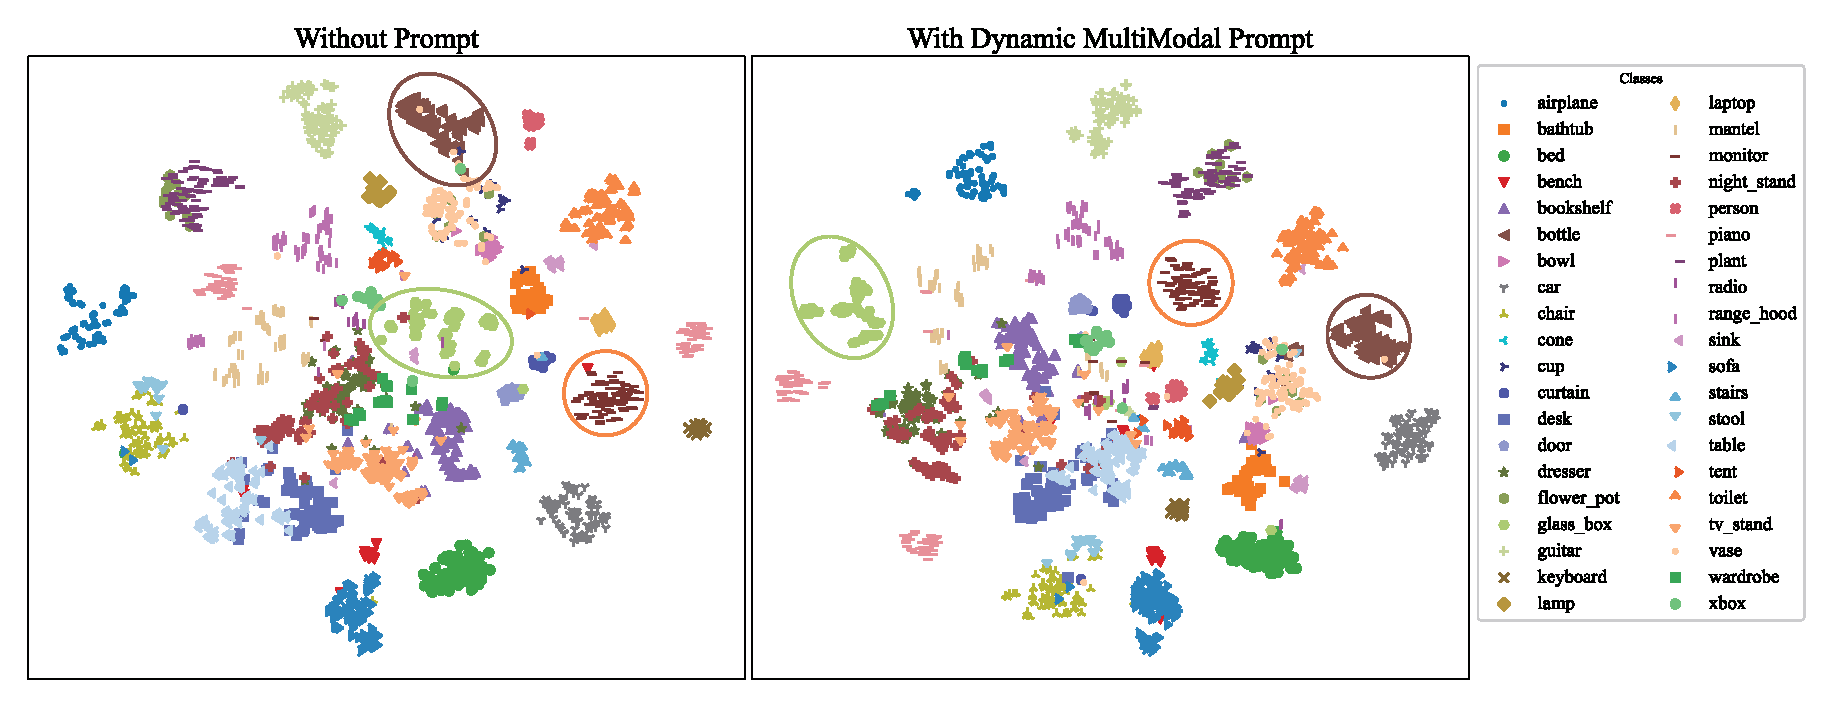
\includegraphics[width=0.9\linewidth]{TSNE.eps}}
% \captionsetup{font={footnotesize}, justification=raggedright}
\caption{The t-SNE visualization of point cloud features in the last layer with or without dynamic multimodal prompt tuning method. We conduct this visualization on few-shot learning with 16-shot and all 40 classes on ModelNet40. The result shows with our dynamic multimodal prompt, features become more distinctively separated.}\label{tsne}
\vspace{4pt}
\end{figure*}
T-SNE visualization is employed to analyze our dynamic multimodal prompt tuning method qualitatively. We extract features from the last layer of the pre-trained point cloud encoder and compare them to the results obtained by directly feeding the point cloud into the point encoder. We choose the standard ModelNet40 dataset, which includes all 40 classes, in a 16-shot, few-shot setting across all classes to perform the t-SNE visualization. The results are shown in Figure~\ref{tsne}.

By integrating dynamic multimodal prompts into the point cloud branch, features become more distinctively separated. For instance, with the prompt, the "glass box" class is now distinctly separated from the "night stand" class, and the "bottle" class is clearly separated from the "vase" class. It is evident that our method enhances the performance of the pre-trained point cloud encoder. 


\section{Ablation Study}\label{ablation}
To explore the architecture design and tuning settings of our proposed DMMPT strategy, we conducted extensive ablation studies in a 16-shot, all-classes few-shot learning setting on ModelNet40.

\subsection{ Evaluating Component Effectiveness in DMMPT}
\begin{table}[ht]
\begin{center}
% \captionsetup{font={footnotesize}, justification=raggedright}
{\caption{Prompt type and accuracy(\%) on ModelNet40 under 16 way all classes few-shot learning setting}\label{table3}}
\begin{tabular}{lcccc}
\toprule
&\multicolumn{1}{c}{text}&\multicolumn{1}{c}{text-point}&\multicolumn{1}{c}{DMMPT}\\
\midrule
\quad acc&88.7&90.3&91.0\\
\bottomrule
\end{tabular}
\end{center}
\end{table}

To assess the effectiveness of each component of our model, we perform experiments on three distinct parts: the text prompt, the text-point prompt, and the dynamic multimodal prompt. The text prompt, referred to as the knowledge collector text part, involves adding static learnable tokens to the text encoder. Building upon this, the text-point prompt utilizes the knowledge collected from the text part and feeds it into the multimodal generator to generate a point cloud prompt for the point cloud encoder. Lastly, we add the knowledge collector image part and evaluate the whole dynamic multimodal prompt. Results are shown in Table~\ref{table3}.

Compared with static text prompt tuning, we observe that multimodal prompts, which integrate text information into the generator of the point cloud prompt, are advantageous. As shown in the Table~\ref{table3}, the text-point prompt achieves a performance gain of 1.6\%. This strengthens the importance of the multimodal generator, which prompts the point cloud encoder and enables information sharing across modalities. Additionally, the dynamic information provided by the image side further enhances performance, resulting in an additional 0.7\% performance gain, showing the efficiency of the dynamic knowledge collector which provides additional dynamic information from other modalities' pre-trained encoders.



\subsection{Multimodal Prompt Size}
Prompt size plays an important role in our method DMMPT, since it reflects the amount of additional knowledge we provide. We conducted experiments across prompt sizes $n\in \{2, \ldots, 11\}$ in the multimodal prompt generator, and the results are illustrated in Figure~\ref{promptSize}. We select a prompt size of 4 in our experiments, as it strikes a balance between performance and parameter efficiency.
\begin{figure}[th]
\centerline{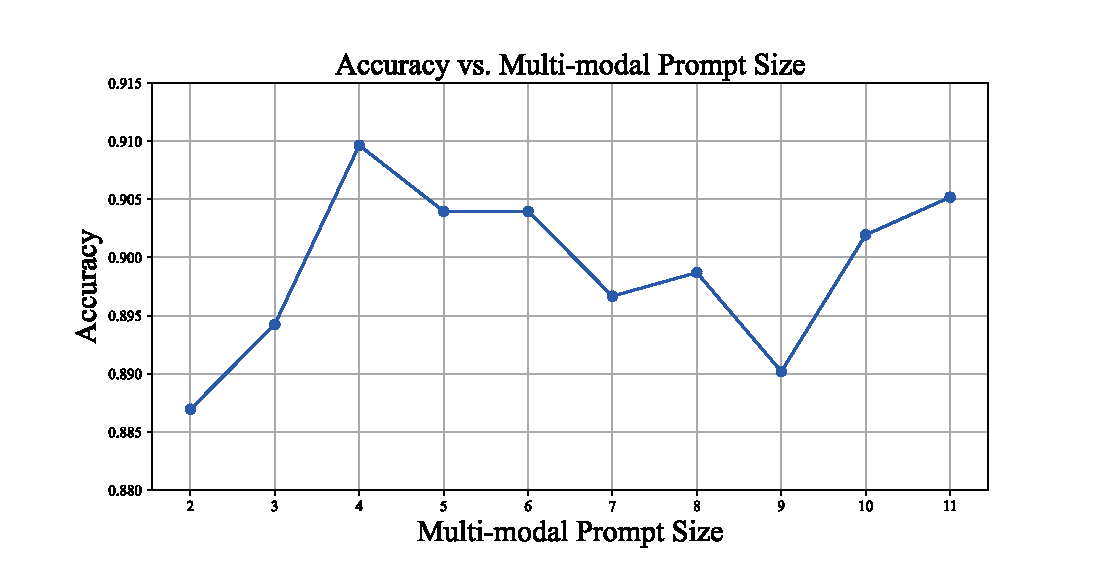
\includegraphics[width=0.9\linewidth]{promptSize.eps}}
% \captionsetup{font={footnotesize}, justification=raggedright}
\caption{Ablation study on prompt size } \label{promptSize}
\vspace{4pt}
\end{figure}
\section{Conclusion}\label{conclusion}
We propose DMMPT, a dynamic multimodal prompt tuning method for significantly boosting the performance of VLM-Guided point cloud models. By introducing a dynamic knowledge collector to obtain additional task-related and data-related knowledge across modalities and using a multimodal prompt generator to enhance the information sharing between encoders, we effectively adapt pre-trained point cloud models to few-shot tasks. Our evaluation extends beyond the standard N-way K-shot few-shot settings to include a more challenging setting with a larger number of classes for model identification. Experiment results consistently demonstrate the outstanding performance of our model across both few-shot learning settings. Our method excels beyond other prompt-based techniques and remains highly competitive with full fine-tuning methods, demonstrating superior computational efficiency.



\begin{ack}This work is supported by the National Natural Science Foundation of China under Grant No.62206128, the National Key Research and Development Program of China under Grant No.2023YFB2703900, the Undergraduate Research Training Program of Nanjing University
of Science and Technology (established in 2023) under Grant No. 2023066001A and Jiangsu Autonomous Driving Technology Innovation and Application Engineering Research Center under Grant No.ZK24-06-02. Our code will be released at https://github.com/eminentgu/DMMPT.
\end{ack}
\bibliography{ref}
\end{document}